% !TeX spellcheck = pl_PL

\rozdzial

%%%%%%%%%%%%%%%%%%%%%%%%%%%%%%%%%%%%%%%%%%%%%%%%%%%%%%%%%%%%%%%%%%%%%%%
\section{Wzorcowanie}
\label{wzorcowanie}

Po lewej stronie okna \textbf{"Wzorcowanie"} program automatycznie podaje wprowadzone wcześniej w części \textbf{"Biuro"} (patrz rozdz. \ref{biuro}) informacje dla danej karty przyjęcia. Podane są: numer zlecenia do którego przypisana jest dana karta (pole \textbf{"Nr zlecenia"}), nazwa zleceniodawcy (pole \textbf{"Zleceniodawca"}) oraz typ i numer fabryczny przyrządu (odpowiednio pola \textbf{"Typ"} i \textbf{"Numer fabryczny"}). 

Pomiędzy poszczególnymi numerami kart można się poruszać albo za pomocą trójkątów przy polu \textbf{"Numer karty"} albo poprzez ręczne wpisanie interesującego nas numeru karty.

Przyciski \textbf{"Poprzednie wzorcowanie"} i \textbf{"Następne wzorcowanie"} przenoszą nas automatycznie do odpowiednio poprzedniego lub następnego wzorcowania danego przyrządu (jeżeli takie istnieją).

\begin{figure}[htb]
	\centering
	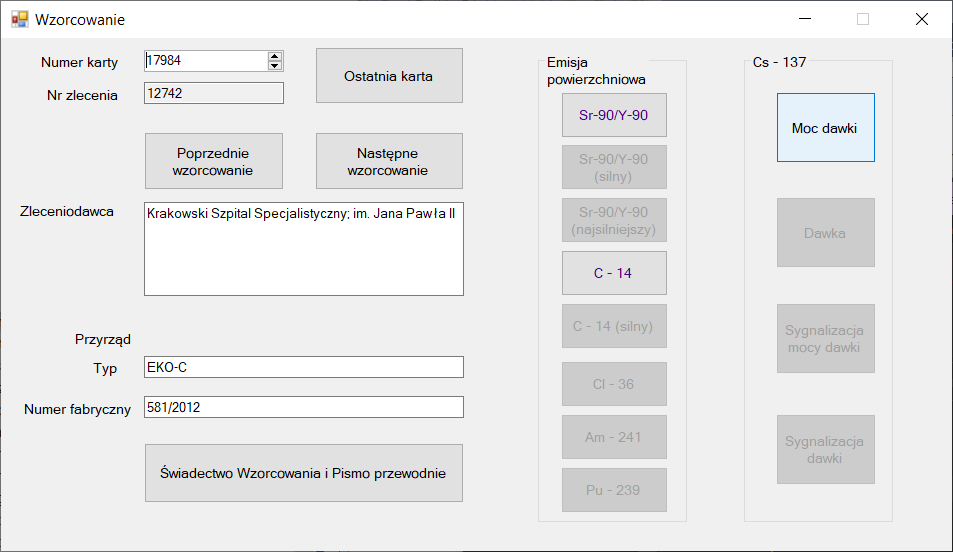
\includegraphics[width=\columnwidth]{obrazki/Wzorcowanie/menu_wzorcowanie.png}
	\caption{Główne okno wzorcowania}
	\label{menuWzorcowanie}
\end{figure}

Wciśnięcie przycisku \textbf{"Ostatnia karta"} powoduje przejście do ostatniego istniejącego w bazie numeru karty. Jeżeli do części \textbf{"Wzorcowanie"} przechodzimy z menu głównego (patrz rozdz. \ref{menuGlowne}) program otwiera się właśnie na ostatniej karcie. W przypadku przejścia za pomocą przycisku \textbf{"Wzorcuj"} z \textbf{"Karty przyjęcia"} (patrz rozdz. \ref{karta_przyjecia}) program podaje dane dla tej konkretnej karty.

Znajdujący się na dole przycisk \textbf{"Świadectwo Wzorcowania i Pismo przewodnie"} powoduje przejście do modułu związanego z przygotowaniem i wydrukiem Świadectwa Wzorcowania i Pisma przewodniego (patrz rozdz. \ref{swiadectwo_pismo}).

Po prawej stronie okna \ref{menuWzorcowanie} znajdują się przyciski pozwalające otworzyć okna związane z konkretnym typem wzorcowania. Dla Cs-137 są to moc dawki, dawka, sygnalizacja mocy dawki i sygnalizacja dawki. W zakresie emisji powierzchniowej dostępne jest jedno z ośmiu źródeł. Dostępność przycisków zależy od zakresu wzorcowania wybranego w procesie wprowadzania karty przyjęcia (patrz rozdz. \ref{karta_przyjecia}).

\subsection{Wzorcowanie w zakresie mocy dawki}
\label{wzorcowanie_moc_dawki}

W górnej części okna znajdują się wypełnione przez program pola \textbf{"Numer karty"}, \textbf{"Arkusz"} oraz \textbf{"Data"}. 

\textbf{TIP:} Za datę wzorcowania program domyślnie przyjmuję datę dzisiejszą, dlatego warto wprowadzać wyniki w dniu pomiaru. Jeżeli wprowadzamy wyniki wzorcowania przeprowadzonego wcześniej, należy pamiętać o zmianie tej daty na tę odpowiadającą pomiarom.

Po prawej stronie znajdują się przyciski \textbf{"Poprzedni arkusz"} i \textbf{"Następny arkusz"} umożliwiające poruszanie się pomiędzy poszczególnymi arkuszami, jeżeli w tym zakresie istnieje więcej niż jeden arkusz (np. wykonujemy pomiary różnymi sondami, lub przy różnych ustawieniach).

Przycisk \textbf{"Dane wzorcowe"} wyświetla dane wzorcowe przeliczone na daną datę i jednostkę.

\textbf{TIP2:} Z przycisku \textbf{"Dane wzorcowe"} warto skorzystać np. w celu ustalenia, w którym punkcie rozpocząć wzorcowanie itp.

\begin{figure}[htb]
	\centering
	\includegraphics[width=\columnwidth]{obrazki/Wzorcowanie/moc_dawki/przyrzad.png}
	\caption{Okno wzorcowania w zakresie mocy dawki - zakładka przyrząd.}
	\label{mocPrzyrzad}
\end{figure}

W menu rozwijanym na górze okna znajdują się opcje umożliwiające podgląd i wydruk dokumentów (w tym przypadku protokołu kalibracyjnego mocy dawki oraz wykresu kalibracyjnego w zakresie mocy dawki) - \textbf{"Dokumenty"} oraz przycisk \textbf{"Zapisz"}, który umożliwia zapisanie częściowych wyników (jeżeli minimalne wymagania są spełnione - wybrany został numer fabryczny sondy).

W zakładce \textbf{"Przyrząd"} (rys. \ref{mocPrzyrzad}) znajdują się wszystkie dane dotyczące wzorcowanego przyrządu. Pola \textbf{"Typ"} oraz \textbf{"Numer fabryczny"} sekcji \textbf{"Przyrząd"} wypełniają się automatycznie danymi wprowadzonymi dla danej karty przyjęcia. Poniżej znajduje się pole \textbf{"Inne nastawy przyrządu"}, do którego należy wprowadzić wszelkie dodatkowe informacje o ustawieniach które mogą mieć wpływ na działanie przyrządu (np. stała czasowa, czułość wejścia itp.). Domyślnie pole to przyjmuje wartość "nie dotyczy".
	
W sekcji sonda należy wypełnić pole \textbf{"Typ"} oraz \textbf{"Numer fabryczny"} sondy. Jeżeli mamy możliwość ustawienia napięcia zasilania sondy, to należy je wpisać w pole \textbf{"Napięcie zasilania sondy"}, w przeciwnym wypadku pozostanie wartość domyślna "nie dotyczy".

\textbf{TIP3:} Należy zwrócić szczególną uwagę na wybór sondy w przypadku przyrządów, które posiadają więcej niż jedną sondę.

W zakładce \textbf{"Warunki"} (rys. \ref{mocWarunki}) przechowywane są informacje o warunkach w jakich odbywało się wzorcowanie. W poszczególnych polach należy podać warunki atmosferyczne sczytane z termohigrobarometru: ciśnienie, temperaturę oraz wilgotność.

Pozostałe ważne dla wzorcowania informacje należy uzupełnić w polu \textbf{"Uwagi"}. Jeżeli przyrząd był wcześniej wzorcowany w laboratorium, program automatycznie wpisuje informację o numerze poprzedniego świadectwa. W tym polu podaje się również takie informacje jak np. czy sygnalizacja przekroczenia zakresu uruchamia się prawidłowo. 

\textbf{TIP4:} W przypadku przyrządów uszkodzonych, w polu \textbf{"Uwagi"} podaje się wszystkie informacje o rodzaju uszkodzenia (np. przyrząd się nie uruchamia, przyrząd nie reaguje na promieniowanie, przyrząd pokazuje to samo wskazanie bez względu na wielkość promieniowania, etc.).

Poniżej znajduje się pole wyboru \textbf{"Przedłużona ważność wzorcowania"}, które należy zaznaczyć, jeżeli przyrząd posiada przedłużoną ważność wzorcowania. Standardowo ważność wzorcowania wynosi rok, jednak w przypadku przyrządów posiadających własne źródło kontrolne ważność ta zostaje przedłużona do dwóch lat.

\begin{figure}[htb]
	\centering
	\includegraphics[width=\columnwidth]{obrazki/Wzorcowanie/moc_dawki/warunki.png}
	\caption{Okno wzorcowania w zakresie mocy dawki - zakładka warunki.}
	\label{mocWarunki}
\end{figure}

Kolejna zakładka to \textbf{"Dane wzorcowe i pomiarowe"}. Tutaj wprowadza się wyniki wzorcowania. Najpierw należy wybrać używany protokół kalibracyjny ławy (lista rozwijana \textbf{"Protokół"}), jednostkę (lista rozwijana \textbf{"Jednostka"}) oraz przypisaną do niej wielkość fizyczną (lista rozwijana \textbf{"Wielkość fizyczna"}). Dzięki tym informacjom i podanej wcześniej dacie wzorcowania program może przygotować dane wzorcowe (dostępne po kliknięciu przycisku \textbf{"Dane wzorcowe"}).

\textbf{TIP5:} Najnowszy protokół kalibracyjny ławy znajduje się na samym dole listy rozwijanej \textbf{"Protokół"}.

\textbf{TIP6:} Po wybraniu jednostki na liście rozwijanej \textbf{"Wielkość fizyczna"} pozostaje jedynie wielkość fizyczna przypisana do tej jednostki. Można jednak dowolnie ją zmienić wpisując inną wielkość fizyczną ręcznie.

\begin{figure}[htb]
	\centering
	\includegraphics[width=\columnwidth]{obrazki/Wzorcowanie/moc_dawki/dane.png}
	\caption{Okno wzorcowania w zakresie mocy dawki - zakładka dane wzorcowe i pomiarowe.}
	\label{mocDane}
\end{figure}

Jako pierwszy wykonujemy pomiar tła. Otrzymaną wartość wpisujemy w polu \textbf{"Tło"}. Następnie szukamy punktu, w którym moc dawki jest jak najbardziej zbliżona do zakresu przyrządu (ale mniejsza od niego). Warto w tym celu posłużyć się danymi wzorcowymi. W tabeli wpisujemy odległość naświetlania oraz numer zastosowanego źródła (1, 2, 3, gdzie 3 to źródło najsilniejsze, a 1 najsłabsze). W kolumnie zakres podajemy zakres, dla którego wykonywany jest pomiar (w przypadku przyrządów z jednym zakresem, jest to cały czas ten sam zakres maksymalny). Mamy dwie opcje wprowadzania wyniku: jedna to bezpośrednie podanie wskazania i jego wahania, druga to podanie maksymalnej i minimalnej wartości wskazanej przez przyrząd. W drugim przypadku program automatycznie wyliczy wskazanie (jako średnią arytmetyczną wartości maksymalnej i minimalnej) oraz wahanie (jako różnicę wyliczonego wskazania i wartości minimalnej).

Aby program podał w tabeli wartości wzorcowe oraz (jeżeli to wymagane) wskazanie i wahanie (z \textbf{"Min"} i \textbf{"Max"}) należy wcisnąć przycisk \textbf{"Oblicz"}. 

\textbf{TIP7:} Jeżeli w danym wierszu tabeli \textbf{"Wartość wzorcowa"} nie zostanie wyświetlona należy sprawdzić podane w tym wierszu odległość i źródło. Brak wyświetlenia wartości wzorcowej oznacza bowiem, że w wybranym protokole nie ma danych wzorcowych dla takiej kombinacji odległość - źródło.

Jeżeli nie ma jakichś szczególnych przesłanek, ay robić inaczej, to kolejne punkty ustalamy tak, aby były 3 punkty na każdy zakres pomiarowy (w przypadku przyrządów posiadających kilka krótszych zakresów pomiarowych), albo aby były co najmniej trzy punkty na dekadę (w przypadku przyrządów o długim zakresie)

Przycisk \textbf{"Dołączyć wszystko"} automatycznie zaznacza wszystkie pola wyboru w kolumnie \textbf{"Dołączyć"}. Kolumna ta wskazuje programowi, które punkty ma brać pod uwagę przy wyliczaniu współczynnika kalibracyjnego oraz jego niepewności. Zdarzają się przyrządu, które w górnej części swojego zakresu ulegają nasyceniu i ich odpowiedź nie jest już proporcjonalna do wielkości pola promieniowania i wtedy zakres takiego przyrządu należy ograniczyć do liniowej części odpowiedzi przyrządu. Drugim przypadkiem, w którym warto zastanowić się nad odłączeniem danego punktu, są punkty w niskich polach promieniowania, których wahanie jest bardzo duże - niewspółmierne do wskazań przyrządu w średnich i wysokich polach promieniowania.

\begin{figure}[htb]
	\centering
	\includegraphics[width=\columnwidth]{obrazki/Wzorcowanie/moc_dawki/wspolczynniki.png}
	\caption{Okno wzorcowania w zakresie mocy dawki - zakładka obliczone współczynniki.}
	\label{mocWspolczynniki}
\end{figure}

W zakładce \textbf{"Obliczone współczynniki"} (rys. \ref{mocWspolczynniki}) znajdują się pola \textbf{"Wykonał(a)"} i \textbf{"Sprawdził(a)"}, w których należy podać odpowiednio dane osoby, która wykonywała wzorcowanie i osoby, która będzie to zatwierdzać. 

\textbf{TIP8:} Program zapamiętuje ostatnio wpisane dane i automatycznie uzupełnia te pola tymi danymi. Należy więc zwrócić na to szczególną uwagę przy zmianie pracownika wykonującego wzorcowanie.

Poniżej znajdują się pola wyboru \textbf{"Dołączyć do świadectwa"} - domyślnie zaznaczone pole oznaczające, że wyniki z tego arkusza mają być zawarte w świadectwie wzorcowania, oraz \textbf{"Poprawa"} - pole wyboru, które należy zaznaczyć jeżeli arkusz jest korektą wcześniejszego wzorcowania (w wydrukach dokumentów numer karty będzie posiadał dodatkową literę \textbf{"P"}).

Przycisk \textbf{"Oblicz"} powoduje wyświetlenie w tabeli wyników wzorcowania dla każdego z zakresów przyrządu. Jeżeli przyrząd był już wzorcowany w zakresie mocy dawki (i w danym zakresie pomiarowym przyrządu), to w dwóch ostatnich kolumnach tabeli pojawią się współczynnik i niepewność z poprzedniego wzorcowania. 

\textbf{TIP9:} Warto zawsze porównać oba wyniki, aby wychwycić ewentualne rozbieżności i spróbować znaleźć ich źródło (czy to błąd we wzorcowaniu, czy np. jakieś uszkodzenie przyrządu).

\subsection{Wzorcowanie w zakresie dawki}
\label{wzorcowanie_dawka)

W górnej części okna znajdują się wypełnione przez program pola \textbf{"Numer karty"}, \textbf{"Arkusz"} oraz \textbf{"Data"}. 

\textbf{TIP:} Za datę wzorcowania program domyślnie przyjmuję datę dzisiejszą, dlatego warto wprowadzać wyniki w dniu pomiaru. Jeżeli wprowadzamy wyniki wzorcowania przeprowadzonego wcześniej, należy pamiętać o zmianie tej daty na tę odpowiadającą pomiarom.

Po prawej stronie znajdują się przyciski \textbf{"Poprzedni arkusz"} i \textbf{"Następny arkusz"} umożliwiające poruszanie się pomiędzy poszczególnymi arkuszami, jeżeli w tym zakresie istnieje więcej niż jeden arkusz (np. wykonujemy pomiary różnymi sondami, lub przy różnych ustawieniach).

Przycisk \textbf{"Dane wzorcowe"} wyświetla dane wzorcowe mocy dawki przeliczone na daną datę i jednostkę.

\textbf{TIP2:} Z przycisku \textbf{"Dane wzorcowe"} warto skorzystać np. w celu ustalenia, w którym punkcie wykonywać naświetlanie przyrządu, jeżeli standardowo stosowana odległość 288,5 cm jest z jakichś przyczyn niedostępna.

\begin{figure}[htb]
	\centering
	\includegraphics[width=\columnwidth]{obrazki/Wzorcowanie/dawka/przyrzad.png}
	\caption{Okno wzorcowania w zakresie dawki - zakładka przyrząd.}
	\label{dawkaPrzyrzad}
\end{figure}

W menu rozwijanym na górze okna znajdują się opcje umożliwiające podgląd i wydruk dokumentów (w tym przypadku protokołu kalibracyjnego dawki oraz wykresu kalibracyjnego w zakresie dawki) - \textbf{"Dokumenty"} oraz przycisk \textbf{"Zapisz"}, który umożliwia zapisanie częściowych wyników (jeżeli minimalne wymagania są spełnione - wybrany został numer fabryczny sondy).

W zakładce \textbf{"Przyrząd"} (rys. \ref{dawkaPrzyrzad}) znajdują się wszystkie dane dotyczące wzorcowanego przyrządu. Pola \textbf{"Typ"} oraz \textbf{"Numer fabryczny"} sekcji \textbf{"Przyrząd"} wypełniają się automatycznie danymi wprowadzonymi dla danej karty przyjęcia. Poniżej znajduje się pole \textbf{"Inne nastawy przyrządu"}, do którego należy wprowadzić wszelkie dodatkowe informacje o ustawieniach które mogą mieć wpływ na działanie przyrządu. Domyślnie pole to przyjmuje wartość "nie dotyczy".

W sekcji sonda należy wypełnić pole \textbf{"Typ"} oraz \textbf{"Numer fabryczny"} sondy. Jeżeli mamy możliwość ustawienia napięcia zasilania sondy, to należy je wpisać w pole \textbf{"Napięcie zasilania sondy"}, w przeciwnym wypadku pozostanie wartość domyślna "nie dotyczy".

\textbf{TIP3:} Należy zwrócić szczególną uwagę na wybór sondy w przypadku przyrządów, które posiadają więcej niż jedną sondę.

\begin{figure}[htb]
	\centering
	\includegraphics[width=\columnwidth]{obrazki/Wzorcowanie/dawka/warunki.png}
	\caption{Okno wzorcowania w zakresie dawki - zakładka warunki.}
	\label{dawkaWarunki}
\end{figure}

W zakładce \textbf{"Warunki"} (rys. \ref{dawkaWarunki}) przechowywane są informacje o warunkach w jakich odbywało się wzorcowanie. W poszczególnych polach należy podać warunki atmosferyczne sczytane z termohigrobarometru: ciśnienie, temperaturę oraz wilgotność.

Pozostałe ważne dla wzorcowania informacje należy uzupełnić w polu \textbf{"Uwagi"}. Jeżeli przyrząd był wcześniej wzorcowany w laboratorium, program automatycznie wpisuje informację o numerze poprzedniego świadectwa. 

\textbf{TIP4:} W przypadku przyrządów uszkodzonych, w polu \textbf{"Uwagi"} podaje się wszystkie informacje o rodzaju uszkodzenia (np. przyrząd się nie uruchamia, przyrząd nie reaguje na promieniowanie, przyrząd pokazuje to samo wskazanie bez względu na wielkość promieniowania, etc.).

Kolejna zakładka to \textbf{"Dane wzorcowe i pomiarowe"} (rys. \ref{dawkaDane}). Tutaj wprowadza się wyniki wzorcowania. Najpierw należy wybrać używany protokół kalibracyjny ławy (lista rozwijana \textbf{"Protokół"}), wybrane źródło (pole \textbf{"Źródło"}) i odległość, na której przyrząd będzie naświetlany (pole \textbf{"Odległość"}). Źródła określone są numerami 1, 2 i 3, gdzie 1 to źródło o najmniejszej mocy dawki, a 3 o największej.

\textbf{TIP5:} Najnowszy protokół kalibracyjny ławy znajduje się na samym dole listy rozwijanej \textbf{"Protokół"}.

\begin{figure}[htb]
	\centering
	\includegraphics[width=\columnwidth]{obrazki/Wzorcowanie/dawka/dane.png}
	\caption{Okno wzorcowania w zakresie dawki - zakładka dane wzorcowe i pomiarowe.}
	\label{dawkaDane}
\end{figure}

Dodatkowo w polu "Zakres" wpisujemy zakres w jakim wzorcujemy. Po prawej stronie na dole mamy możliwość wyboru jednej z czterech wielkości fizycznych:
\begin{itemize}
	\item indywidualnego równoważnika dawki $H_{p}(10)$
	\item indywidualnego równoważnika dawki $H_{p}(0,07)$
	\item indywidualnego równoważnika dawki $H^{*}$
	\item mocy kermy
\end{itemize}

W pierwszej kolumnie tabeli wpisujemy kolejne dawki jakimi zamierzamy naświetlić wzorcowany dawkomierz. Standardowo stosowane są dawki: 0,1; 0,2; 0,4; 0,8; 1,6; 3,2 oraz 6,4 mSv. Następnie wciskając znajdujący się po prawej stronie przycisk \textbf{"Licz"} otrzymujemy w tabeli czasy jakie są wymagane, aby dokonać ekspozycji przyrządu zadaną dawką na wybranej wcześniej odległości i przy użyciu podanego źródła.

\textbf{TIP6:} Program zakłada, że kolejne dawki są sumowane, więc podaje czasy potrzebne do naświetlenia przyrządu dawką o wartości równej różnicy między dawką zadaną, a dawką poprzednią.

W trzeciej kolumnie podajemy wartości dawki wskazane po naświetleniu przez wzorcowany przyrząd.

Przycisk \textbf{"Dołącz wszystko"} automatycznie zaznacza wszystkie pola wyboru w kolumnie \textbf{"Dołączyć"}. Kolumna ta wskazuje programowi, które punkty ma brać pod uwagę przy wyliczaniu współczynnika kalibracyjnego oraz jego niepewności.

\begin{figure}[htb]
	\centering
	\includegraphics[width=\columnwidth]{obrazki/Wzorcowanie/dawka/wspolczynniki.png}
	\caption{Okno wzorcowania w zakresie dawki - zakładka obliczone współczynniki.}
	\label{dawkaWspolczynniki}
\end{figure}

W zakładce \textbf{"Obliczone współczynniki"} (rys. \ref{dawkaWspolczynniki}) znajdują się pola \textbf{"Wykonał(a)"} i \textbf{"Sprawdził(a)"}, w których należy podać odpowiednio dane osoby, która wykonywała wzorcowanie i osoby, która będzie to zatwierdzać. 

\textbf{TIP7:} Program zapamiętuje ostatnio wpisane dane i automatycznie uzupełnia te pola tymi danymi. Należy więc zwrócić na to szczególną uwagę przy zmianie pracownika wykonującego wzorcowanie.

Poniżej znajduje się pole wyboru \textbf{"Dołączyć do świadectwa"} - domyślnie zaznaczone pole oznaczające, że wyniki z tego arkusza mają być zawarte w świadectwie wzorcowania.

Przycisk \textbf{"Oblicz"} powoduje wyświetlenie wyników wzorcowania. Jeżeli przyrząd był już wzorcowany w zakresie dawki, to w polach po prawej stronie pojawią się współczynnik i niepewność z poprzedniego wzorcowania. 

\textbf{TIP8:} Warto zawsze porównać oba wyniki, aby wychwycić ewentualne rozbieżności i spróbować znaleźć ich źródło (czy to błąd we wzorcowaniu, czy np. jakieś uszkodzenie przyrządu).

\subsection{Wzorcowanie w zakresie sygnalizacji mocy dawki}
\label{wzorcowanie_syg_moc)
		
	\begin{figure}[H]
		\centering
		\includegraphics[width=\columnwidth]{obrazki/Wzorcowanie/syg_mocy_dawki/przyrzad.png}
		\caption{Okno wzorcowania w zakresie sygnalizacji mocy dawki - zakładka przyrząd.}
		\label{sygMocyPrzyrzad}
	\end{figure}

	W górnej części okna znajdują się wypełnione przez program pola \textbf{"Numer karty"}, \textbf{"Arkusz"} oraz \textbf{"Data"}. 
	
	\textbf{TIP:} Za datę wzorcowania program domyślnie przyjmuję datę dzisiejszą, dlatego warto wprowadzać wyniki w dniu pomiaru. Jeżeli wprowadzamy wyniki wzorcowania przeprowadzonego wcześniej, należy pamiętać o zmianie tej daty na tę odpowiadającą pomiarom.
	
	Po prawej stronie znajdują się przyciski \textbf{"Poprzedni arkusz"} i \textbf{"Następny arkusz"} umożliwiające poruszanie się pomiędzy poszczególnymi arkuszami, jeżeli w tym zakresie istnieje więcej niż jeden arkusz (np. wykonujemy pomiary różnymi sondami, lub przy różnych ustawieniach).
	
	Przycisk \textbf{"Dane wzorcowe"} wyświetla dane wzorcowe mocy dawki przeliczone na daną datę i jednostkę.
	
	\textbf{TIP2:} Z przycisku \textbf{"Dane wzorcowe"} warto skorzystać np. w celu ustalenia na jakiej odległości i przy użyciu którego ze źródeł warto rozpocząć wzorcowanie.
	
	\begin{figure}[htb]
	\centering
	\includegraphics[width=\columnwidth]{obrazki/Wzorcowanie/syg_mocy_dawki/warunki.png}
	\caption{Okno wzorcowania w zakresie sygnalizacji mocy dawki - zakładka warunki.}
	\label{sygMocyWarunki}
	\end{figure}
	
	W menu rozwijanym na górze okna znajdują się opcje umożliwiające podgląd i wydruk dokumentów (w tym przypadku protokołu kalibracyjnego sygnalizacji mocy dawki) - \textbf{"Dokumenty"} oraz przycisk \textbf{"Zapisz"}, który umożliwia zapisanie częściowych wyników (jeżeli minimalne wymagania są spełnione - wybrany został numer fabryczny sondy).
	
	W zakładce \textbf{"Przyrząd"} (rys. \ref{sygMocyPrzyrzad}) znajdują się wszystkie dane dotyczące wzorcowanego przyrządu. Pola \textbf{"Typ"} oraz \textbf{"Numer fabryczny"} sekcji \textbf{"Przyrząd"} wypełniają się automatycznie danymi wprowadzonymi dla danej karty przyjęcia. Poniżej znajduje się pole \textbf{"Inne nastawy przyrządu"}, do którego należy wprowadzić wszelkie dodatkowe informacje o ustawieniach które mogą mieć wpływ na działanie przyrządu. Domyślnie pole to przyjmuje wartość "nie dotyczy".
	
	W sekcji sonda należy wypełnić pole \textbf{"Typ"} oraz \textbf{"Numer fabryczny"} sondy. Jeżeli mamy możliwość ustawienia napięcia zasilania sondy, to należy je wpisać w pole \textbf{"Napięcie zasilania sondy"}, w przeciwnym wypadku pozostanie wartość domyślna "nie dotyczy".
	
	\textbf{TIP3:} Należy zwrócić szczególną uwagę na wybór sondy w przypadku przyrządów, które posiadają więcej niż jedną sondę.
	
	\begin{figure}[htb]
	\centering
	\includegraphics[width=\columnwidth]{obrazki/Wzorcowanie/syg_mocy_dawki/dane.png}
	\caption{Okno wzorcowania w zakresie sygnalizacji mocy dawki - zakładka dane wzorcowe i pomiarowe.}
	\label{sygMocyDane}
	\end{figure}
	
	W zakładce \textbf{"Warunki"} (rys. \ref{sygMocyWarunki}) przechowywane są informacje o warunkach w jakich odbywało się wzorcowanie. W poszczególnych polach należy podać warunki atmosferyczne sczytane z termohigrobarometru: ciśnienie, temperaturę oraz wilgotność.
	
	Pozostałe ważne dla wzorcowania informacje należy uzupełnić w polu \textbf{"Uwagi"}. Jeżeli przyrząd był wcześniej wzorcowany w laboratorium, program automatycznie wpisuje informację o numerze poprzedniego świadectwa. 
	
	\textbf{TIP4:} W przypadku przyrządów uszkodzonych, w polu \textbf{"Uwagi"} podaje się wszystkie informacje o rodzaju uszkodzenia (np. przyrząd się nie uruchamia, przyrząd nie reaguje na promieniowanie, przyrząd pokazuje to samo wskazanie bez względu na wielkość promieniowania, etc.).

	Kolejna zakładka to \textbf{"Dane wzorcowe i pomiarowe"} (rys. \ref{sygMocyDane}). Tutaj wprowadza się wyniki wzorcowania. Najpierw należy wybrać używany protokół kalibracyjny ławy (lista rozwijana \textbf{"Protokół"}) oraz jednostkę (lista rozwijana \textbf{"Jednostka"}).
	
	\textbf{TIP5:} Najnowszy protokół kalibracyjny ławy znajduje się na samym dole listy rozwijanej \textbf{"Protokół"}.
	
	\begin{figure}[htb]
	\centering
	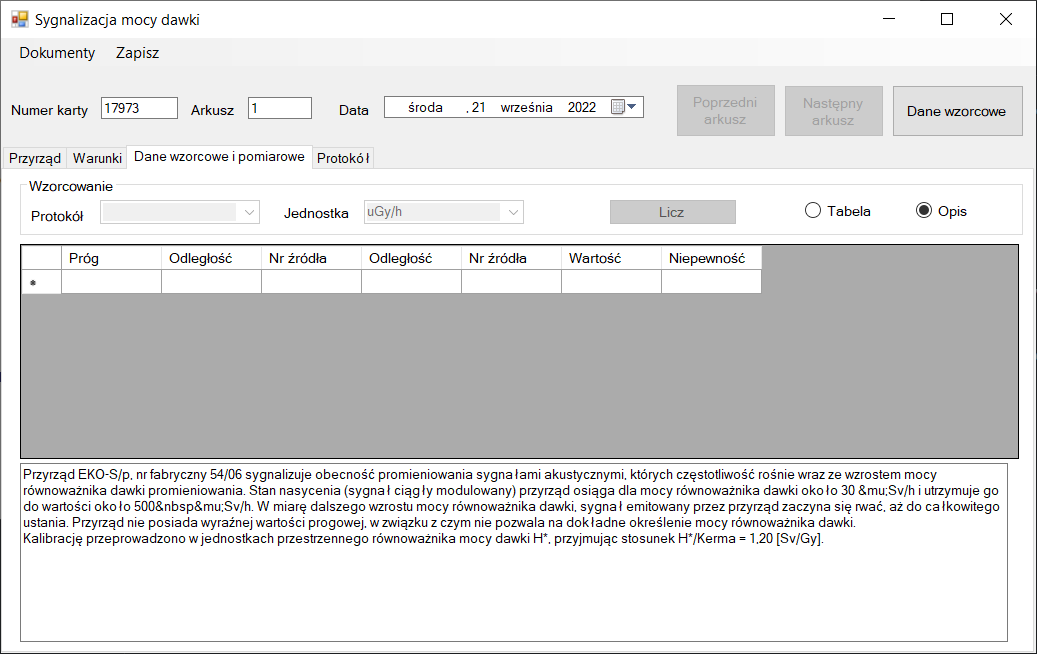
\includegraphics[width=\columnwidth]{obrazki/Wzorcowanie/syg_mocy_dawki/dane2.png}
	\caption{Okno wzorcowania w zakresie sygnalizacji mocy dawki - zakładka dane wzorcowe i pomiarowe.}
	\label{sygMocyDane2}
\end{figure}

	Po prawej stronie mamy do wyboru dwie opcje uzupełniania wyników: \textbf{"Tabela"} lub \textbf{"Opis"}. Wybieramy jedną w zależności od wzorcowanego typu przyrządu. 
		
	W pierwszej kolumnie tabeli podajemy ustawiony na przyrządzie próg sygnalizacji mocy dawki. Naświetlanie przyrządu rozpoczynamy od punktu i źródła, przy których moc dawki jest niższa niż ustawiony próg. (W tym celu warto skorzystać z przycisku \textbf{"Dane wzorcowe"}). Następnie powoli przesuwamy się w kierunku wzrastających mocy dawek. W kolumnie drugiej i trzeciej podajemy odpowiednio odległość i numer źródła, przy których uruchomiła się sygnalizacja ostrzegawcza przyrządu. Następnie przesuwamy przyrząd w kierunku malejących mocy dawek i obserwujemy, kiedy nastąpi wyłączenie sygnalizacji ostrzegawczej. W kolumnach cztery i pięć podajemy odległość i numer źródła, przy których to nastąpiło. Następnie wciskając znajdujący się po prawej stronie przycisk \textbf{"Licz"} otrzymujemy wyliczoną rzeczywistą wartość, przy której uruchamia się sygnalizacja ostrzegawcza wraz z niepewnością (dwie ostatnie kolumny tabeli).

W przypadku opcji \textbf{"Opis"} (rys. \ref{sygMocyDane2}) wykonujemy opis zachowania przyrządu w polu promieniowania.
	
	\begin{figure}[htb]
		\centering
		\includegraphics[width=\columnwidth]{obrazki/Wzorcowanie/syg_mocy_dawki/wspolczynniki.png}
		\caption{Okno wzorcowania w zakresie sygnalizacji mocy dawki - zakładka obliczone współczynniki.}
		\label{sygMocyWspolczynniki}
	\end{figure}
	
	W zakładce \textbf{"Obliczone współczynniki"} (rys. \ref{sygMocyWspolczynniki}) znajdują się pola \textbf{"Wykonał(a)"} i \textbf{"Sprawdził(a)"}, w których należy podać odpowiednio dane osoby, która wykonywała wzorcowanie i osoby, która będzie to zatwierdzać. 
	
	\textbf{TIP7:} Program zapamiętuje ostatnio wpisane dane i automatycznie uzupełnia te pola tymi danymi. Należy więc zwrócić na to szczególną uwagę przy zmianie pracownika wykonującego wzorcowanie.
	
	Poniżej znajduje się pole wyboru \textbf{"Dołączyć"} - domyślnie zaznaczone pole oznaczające, że wyniki z tego arkusza mają być zawarte w świadectwie wzorcowania.

\subsection{Wzorcowanie w zakresie sygnalizacji dawki}
\label{wzorcowanie_syg_moc)
	
	W górnej części okna znajdują się wypełnione przez program pola \textbf{"Numer karty"}, \textbf{"Arkusz"} oraz \textbf{"Data"}. 
	
	\textbf{TIP:} Za datę wzorcowania program domyślnie przyjmuję datę dzisiejszą, dlatego warto wprowadzać wyniki w dniu pomiaru. Jeżeli wprowadzamy wyniki wzorcowania przeprowadzonego wcześniej, należy pamiętać o zmianie tej daty na tę odpowiadającą pomiarom.
	
	\begin{figure}[htb]
		\centering
		\includegraphics[width=\columnwidth]{obrazki/Wzorcowanie/syg_dawki/przyrzad.png}
		\caption{Okno wzorcowania w zakresie sygnalizacji dawki - zakładka przyrząd.}
		\label{sygDawkiPrzyrzad}
	\end{figure}
	
	Po prawej stronie znajdują się przyciski \textbf{"Poprzedni arkusz"} i \textbf{"Następny arkusz"} umożliwiające poruszanie się pomiędzy poszczególnymi arkuszami, jeżeli w tym zakresie istnieje więcej niż jeden arkusz (np. wykonujemy pomiary różnymi sondami, lub przy różnych ustawieniach).
	
	Przycisk \textbf{"Dane wzorcowe"} wyświetla dane wzorcowe mocy dawki przeliczone na daną datę i jednostkę.
	
	\textbf{TIP2:} Z przycisku \textbf{"Dane wzorcowe"} warto skorzystać np. w celu ustalenia, w którym punkcie wykonywać naświetlanie przyrządu, jeżeli standardowo stosowana odległość 288,5 cm jest z jakichś przyczyn niedostępna.
	
	W menu rozwijanym na górze okna znajdują się opcje umożliwiające podgląd i wydruk dokumentów (w tym przypadku protokołu kalibracyjnego sygnalizacji dawki) - \textbf{"Dokumenty"} oraz przycisk \textbf{"Zapisz"}, który umożliwia zapisanie częściowych wyników (jeżeli minimalne wymagania są spełnione - wybrany został numer fabryczny sondy).
	
	\begin{figure}[htb]
		\centering
		\includegraphics[width=\columnwidth]{obrazki/Wzorcowanie/syg_dawki/warunki.png}
		\caption{Okno wzorcowania w zakresie sygnalizacji dawki - zakładka warunki.}
		\label{sygDawkiWarunki}
	\end{figure}
	
	W zakładce \textbf{"Przyrząd"} (rys. \ref{sygDawkiPrzyrzad}) znajdują się wszystkie dane dotyczące wzorcowanego przyrządu. Pola \textbf{"Typ"} oraz \textbf{"Numer fabryczny"} sekcji \textbf{"Przyrząd"} wypełniają się automatycznie danymi wprowadzonymi dla danej karty przyjęcia. Poniżej znajduje się pole \textbf{"Inne nastawy przyrządu"}, do którego należy wprowadzić wszelkie dodatkowe informacje o ustawieniach które mogą mieć wpływ na działanie przyrządu. Domyślnie pole to przyjmuje wartość "nie dotyczy".
	
	W sekcji sonda należy wypełnić pole \textbf{"Typ"} oraz \textbf{"Numer fabryczny"} sondy. Jeżeli mamy możliwość ustawienia napięcia zasilania sondy, to należy je wpisać w pole \textbf{"Napięcie zasilania sondy"}, w przeciwnym wypadku pozostanie wartość domyślna "nie dotyczy".
	
	\textbf{TIP3:} Należy zwrócić szczególną uwagę na wybór sondy w przypadku przyrządów, które posiadają więcej niż jedną sondę.
	
	W zakładce \textbf{"Warunki"} (rys. \ref{sygDawkiWarunki}) przechowywane są informacje o warunkach w jakich odbywało się wzorcowanie. W poszczególnych polach należy podać warunki atmosferyczne sczytane z termohigrobarometru: ciśnienie, temperaturę oraz wilgotność.

	Pozostałe ważne dla wzorcowania informacje należy uzupełnić w polu \textbf{"Uwagi"}. Jeżeli przyrząd był wcześniej wzorcowany w laboratorium, program automatycznie wpisuje informację o numerze poprzedniego świadectwa. 
	
	\begin{figure}[htb]
		\centering
		\includegraphics[width=\columnwidth]{obrazki/Wzorcowanie/syg_dawki/dane.png}
		\caption{Okno wzorcowania w zakresie sygnalizacji dawki - zakładka dane wzorcowe i pomiarowe.}
		\label{sygDawkiDane}
	\end{figure}
	
	\textbf{TIP4:} W przypadku przyrządów uszkodzonych, w polu \textbf{"Uwagi"} podaje się wszystkie informacje o rodzaju uszkodzenia (np. przyrząd się nie uruchamia, przyrząd nie reaguje na promieniowanie, przyrząd pokazuje to samo wskazanie bez względu na wielkość promieniowania, etc.).
	
	Kolejna zakładka to \textbf{"Dane wzorcowe i pomiarowe"} (rys. \ref{dawkaDane}). Tutaj wprowadza się wyniki wzorcowania. Najpierw należy wybrać używany protokół kalibracyjny ławy (lista rozwijana \textbf{"Protokół"}), wybrane źródło (pole \textbf{"Źródło"}) i odległość, na której przyrząd będzie naświetlany (pole \textbf{"Odległość"}). Źródła określone są numerami 1, 2 i 3, gdzie 1 to źródło o najmniejszej mocy dawki, a 3 o największej.
	
	\textbf{TIP5:} Najnowszy protokół kalibracyjny ławy znajduje się na samym dole listy rozwijanej \textbf{"Protokół"}.
	
	Następnie z listy rozwijanej \textbf{"Jednostka"} należy wybrać jednostkę mocy dawki odpowiadającą jednostce dawki, w jakiej wyskalowany jest przyrząd. Np. jeżeli jednostka przyrządu na mSv, to z listy rozwianej należy wybrać mSv/h.
	
	\begin{figure}[htb]
		\centering
		\includegraphics[width=\columnwidth]{obrazki/Wzorcowanie/syg_dawki/wspolczynniki.png}
		\caption{Okno wzorcowania w zakresie sygnalizacji dawki - zakładka obliczone współczynniki.}
		\label{sygDawkiWspolczynniki}
	\end{figure}
	
	W pierwszej kolumnie tabeli podajemy ustawiony na przyrządzie próg sygnalizacji dawki. Naciskając przycisk \textbf{"Licz"} otrzymujemy w drugiej kolumnie (\textbf{"Czas wzorcowy"}) informację o czasie wzorcowym w jakim przyrząd (danym źródłem, na danej odległości) będzie naświetlony zadaną dawką. Ułatwia to kalibrację, gdyż wzorcujący wie, kiedy powinien się spodziewać uruchomienia sygnalizacji przyrządu. Następnie należy włączyć naświetlanie i zmierzyć stoperem czas po jakim uruchomiona zostanie sygnalizacja ostrzegawcza. Zmierzony czas notujemy w kolumnie trzeciej (\textbf{"Czas zmierzony"}). Naciskając powtórnie ten sam przycisk \textbf{"Licz"} otrzymujemy w kolumnie czwartej rzeczywistą wartość, przy której włączona zostaje sygnalizacja ostrzegawcza. W ostatniej kolumnie tabeli należy zanotować wskazanie przyrządu.
	
	W zakładce \textbf{"Obliczone współczynniki"} (rys. \ref{sygDawkiWspolczynniki}) znajdują się pola \textbf{"Wykonał(a)"} i \textbf{"Sprawdził(a)"}, w których należy podać odpowiednio dane osoby, która wykonywała wzorcowanie i osoby, która będzie to zatwierdzać. 
	
	\textbf{TIP7:} Program zapamiętuje ostatnio wpisane dane i automatycznie uzupełnia te pola tymi danymi. Należy więc zwrócić na to szczególną uwagę przy zmianie pracownika wykonującego wzorcowanie.
	
	Poniżej znajduje się pole wyboru \textbf{"Dołączyć"} - domyślnie zaznaczone pole oznaczające, że wyniki z tego arkusza mają być zawarte w świadectwie wzorcowania.

\subsection{Wzorcowanie w zakresie emisji powierzchniowej}
\label{wzorcowanie_emisja}

	W górnej części okna znajdują się wypełnione przez program pola \textbf{"Numer karty"}, \textbf{"Arkusz"} oraz \textbf{"Data"} oraz \textbf{"Źródło"}. 
	
	\textbf{TIP:} Za datę wzorcowania program domyślnie przyjmuję datę dzisiejszą, dlatego warto wprowadzać wyniki w dniu pomiaru. Jeżeli wprowadzamy wyniki wzorcowania przeprowadzonego wcześniej, należy pamiętać o zmianie tej daty na tę odpowiadającą pomiarom.
	
	Z listy rozwijanej \textbf{"Jednostka"} należy wybrać jednostkę, w jakiej wyskalowany jest przyrząd.
	
	Po prawej stronie znajdują się przyciski \textbf{"Poprzedni arkusz"} i \textbf{"Następny arkusz"} umożliwiające poruszanie się pomiędzy poszczególnymi arkuszami, jeżeli w tym zakresie istnieje więcej niż jeden arkusz (np. wykonujemy pomiary różnymi sondami, lub przy różnych ustawieniach).
	
	\begin{figure}[htb]
		\centering
		\includegraphics[width=\columnwidth]{obrazki/Wzorcowanie/emisja/przyrzad.png}
		\caption{Okno wzorcowania w zakresie emisji powierzchniowej - zakładka przyrząd.}
		\label{emisjaPrzyrzad}
	\end{figure}
	
	W zakładce \textbf{"Przyrząd"} (rys. \ref{emisjaPrzyrzad}) znajdują się wszystkie dane dotyczące wzorcowanego przyrządu. Pola \textbf{"Typ"} oraz \textbf{"Numer fabryczny"} sekcji \textbf{"Przyrząd"} wypełniają się automatycznie danymi wprowadzonymi dla danej karty przyjęcia. Poniżej znajduje się pole \textbf{"Zakres"}, które należy uzupełnić jeżeli przyrząd posiada więcej niż jeden zakres pomiarowy. Domyślnie pole to przyjmuje wartość "nie dotyczy". Pole \textbf{"Inne nastawy przyrządu"}, służy do podania wszelkich dodatkowych informacji o ustawieniach, które mogą mieć wpływ na działanie przyrządu (np. stała czasowa, czułość wejścia itp.). Domyślnie pole to przyjmuje wartość "nie dotyczy".
	
	W sekcji sonda należy wypełnić pole \textbf{"Typ"} oraz \textbf{"Numer fabryczny"} sondy. Jeżeli mamy możliwość ustawienia napięcia zasilania sondy, to należy je wpisać w pole \textbf{"Napięcie zasilania sondy"}, w przeciwnym wypadku pozostanie wartość domyślna "nie dotyczy".
	
	Przycisk \textbf{"Znajdź dostępne typy sond"} wyszukuje w bazie danych wszystkie sondy przypisane do przyrządu.
	
	\textbf{TIP3:} Należy zwrócić szczególną uwagę na wybór sondy w przypadku przyrządów, które posiadają więcej niż jedną sondę.
	
	W zakładce \textbf{"Warunki"} (rys. \ref{emisjaWarunki}) przechowywane są informacje o warunkach w jakich odbywało się wzorcowanie. W poszczególnych polach należy podać warunki atmosferyczne sczytane z termohigrobarometru: ciśnienie, temperaturę oraz wilgotność.
	
	W części \textbf{"Inne"} podajemy informcje o zastosowanej podstawce (pole \textbf{"Podstawka"}), odległości sondy od źródła promieniowania (pole \textbf{"Odległość źródło - sonda"}) oraz o współczynniku korekcyjnym związanym z zastosowaną podstawką (pole \textbf{"Współczynnik korekcyjny"}). W przypadku braku podstawki współczynnik ten przyjmuje wartość 1.
	
	Pozostałe ważne dla wzorcowania informacje należy uzupełnić w polu \textbf{"Uwagi"}. Jeżeli przyrząd był wcześniej wzorcowany w laboratorium, program automatycznie wpisuje informację o numerze poprzedniego świadectwa.  
	
	\textbf{TIP4:} W przypadku przyrządów uszkodzonych, w polu \textbf{"Uwagi"} podaje się wszystkie informacje o rodzaju uszkodzenia (np. przyrząd się nie uruchamia, przyrząd nie reaguje na promieniowanie, przyrząd pokazuje to samo wskazanie bez względu na wielkość promieniowania, etc.).
	
	\begin{figure}[htb]
		\centering
		\includegraphics[width=\columnwidth]{obrazki/Wzorcowanie/emisja/warunki.png}
		\caption{Okno wzorcowania w zakresie emisji powierzchniowej - zakładka warunki.}
		\label{emisjaWarunki}
	\end{figure}
	
	Kolejna zakładka to \textbf{"Dane wzorcowe i pomiarowe"}. Tutaj wprowadza się wyniki wzorcowania. Wyniki pomiarów tła należy wprowadzić w drugiej kolumnie tabeli. Wyniki pomiarów z użyciem źródła można albo wprowadzić w formie gotowych wyników w pierwszej kolumnie (\textbf{"Wskazanie"}), albo podać minimalną i maksymalną wartość wskazywaną przez przyrząd odpowiednio w kolumnach trzeciej i czwartej (kolumny \textbf{"Min"} i \textbf{"Max"}). W drugim przypadku program automatycznie wyliczy wskazanie (jako średnią arytmetyczną wartości maksymalnej i minimalnej) oraz wahanie (jako różnicę wyliczonego wskazania i wartości minimalnej).
	
	\begin{figure}[htb]
		\centering
		\includegraphics[width=\columnwidth]{obrazki/Wzorcowanie/emisja/dane.png}
		\caption{Okno wzorcowania w zakresie emisji powierzchniowej- zakładka dane wzorcowe i pomiarowe.}
		\label{emisjaDane}
	\end{figure}
	
	\begin{figure}[htb]
		\centering
		\includegraphics[width=\columnwidth]{obrazki/Wzorcowanie/emisja/wspolczynniki.png}
		\caption{Okno wzorcowania w zakresie emisji powierzchniowej - zakładka obliczone współczynniki.}
		\label{emisjaWspolczynniki}
	\end{figure}
	
	W zakładce \textbf{"Obliczone współczynniki"} (rys. \ref{emisjaWspolczynniki}) znajdują się pola \textbf{"Wykonał(a)"} i \textbf{"Sprawdził(a)"}, w których należy podać odpowiednio dane osoby, która wykonywała wzorcowanie i osoby, która będzie to zatwierdzać. 
	
	\textbf{TIP5:} Program zapamiętuje ostatnio wpisane dane i automatycznie uzupełnia te pola tymi danymi. Należy więc zwrócić na to szczególną uwagę przy zmianie pracownika wykonującego wzorcowanie.
	
	Poniżej znajduje się pole wyboru \textbf{"Dołączyć do świadectwa"} - domyślnie zaznaczone pole oznaczające, że wyniki z tego arkusza mają być zawarte w świadectwie wzorcowania.
	
	Przycisk \textbf{"Oblicz"} powoduje wyświetlenie wyników wzorcowania. Jeżeli przyrząd był już wzorcowany w zakresie dawki, to w polach po prawej stronie pojawią się współczynnik i niepewność z poprzedniego wzorcowania. 
	
	\textbf{TIP6:} Warto zawsze porównać oba wyniki, aby wychwycić ewentualne rozbieżności i spróbować znaleźć ich źródło (czy to błąd we wzorcowaniu, czy np. jakieś uszkodzenie przyrządu). Współczynnik kalibracyjny nie powinien się różnić od jego poprzedniej wartości o więcej niż 20 procent.

\subsection{Świadectwo i pismo przewodnie}
\label{swiadectwo_pismo}

	Do tego okna (rys. \ref{menuSwiadectwo}) należy przejść po zakończeniu wszystkich wzorcowań danego przyrządu. Tutaj przygotowuje się do wydruku Świadectwo Wzorcowania oraz pismo przewodnie. 
	
	Na górze okna znajdują się pola \textbf{"Autoryzował(a)"}, \textbf{"Nr pisma"}, \textbf{"Data wykonania"} i \textbf{"Data wydania"}. Są one wstępnie wypełnione przez program. Program zapamiętuje ostatnio wpisaną osobę w polu \textbf{"Autoryzował(a)"} i automatycznie uzupełnia to pole zapamiętanymi danymi. Proponowany przez program numer pisma jest o jeden większy od ostatniego zapisanego w bazie danych numeru pisma. Za datę wykonania oraz datę wydania program domyślnie przyjmuję datę dzisiejszą.

	W zakładce \textbf{"Obliczone współczynniki"} (rys. \ref{emisjaWspolczynniki}) znajdują się pola \textbf{"Wykonał(a)"} i \textbf{"Sprawdził(a)"}, w których należy podać odpowiednio dane osoby, która wykonywała wzorcowanie i osoby, która będzie to zatwierdzać. 

	TIP: Wszystkie powyższe dane są uzupełniane przez program po zrobieniu odpowiednich założeń (np. że wystawiamy dokumenty w ten sam dzień, w którym było wykonane wzorcowanie), dlatego zawsze należy sprawdzić ich zgodność ze stanem faktycznym.
	
	Po prawej stronie znajdują się dwa pola wyboru: \textbf{"Poprawa"} oraz \textbf{"Przedłużona ważność wzorcowania"}. \textbf{"Poprawa"} jest to pole wyboru, które należy zaznaczyć jeżeli Świadectwo Wzorcowania jest korektą wcześniejszego Świadectwa (w wydrukach dokumentów numer karty będzie posiadał dodatkową literę \textbf{"P"}). Pole \textbf{"Przedłużona ważność wzorcowania"}, należy zaznaczyć, jeżeli przyrząd posiada przedłużoną ważność wzorcowania. Standardowo ważność wzorcowania wynosi rok, jednak w przypadku przyrządów posiadających własne źródło kontrolne ważność ta zostaje przedłużona do dwóch lat.

	\begin{figure}[htb]
		\centering
		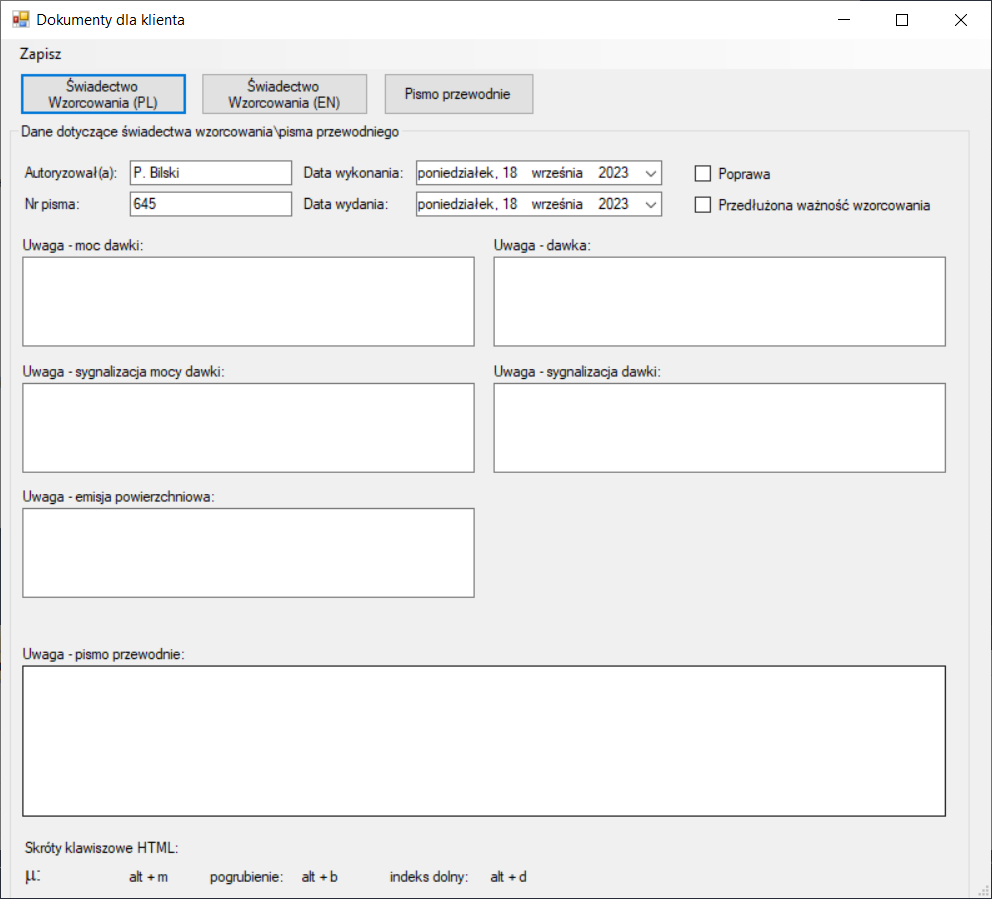
\includegraphics[width=\columnwidth]{obrazki/Wzorcowanie/menu_swiadectwo.png}
		\caption{Menu główne przygotowania i wydruku dokumentów.}
		\label{menuSwiadectwo}
	\end{figure}

	Główną część okna zajmują pola, w których możemy zamieścić uwagi do poszczególnych wyników wzorcowań albo do pisma przewodniego:
	\begin{itemize}
		\item \textbf{Uwaga - moc dawki} - pole do zamieszczenia uwagi, która umieszczona będzie na Świadectwie Wzorcowania w części dotyczącej wzorcowania w zakresie mocy dawki
		\item \textbf{Uwaga - dawka} - pole do zamieszczenia uwagi, która umieszczona będzie na Świadectwie Wzorcowania w części dotyczącej wzorcowania w zakresie dawki
		\item \textbf{Uwaga - sygnalizacja mocy dawki} - pole do zamieszczenia uwagi, która umieszczona będzie na Świadectwie Wzorcowania w części dotyczącej wzorcowania w zakresie sygnalizacji mocy dawki
		\item \textbf{Uwaga - sygnalizacja dawki} - pole do zamieszczenia uwagi, która umieszczona będzie na Świadectwie Wzorcowania w części dotyczącej wzorcowania w zakresie sygnalizacji dawki
		\item \textbf{Uwaga - emisja powierzchniowa} - pole do zamieszczenia uwagi, która umieszczona będzie na Świadectwie Wzorcowania w części dotyczącej wzorcowania w zakresie emisji powierzchniowej
		\item \textbf{Uwaga - pismo przewodnie} - pole do zamieszczenia uwagi, która umieszczona będzie na piśmie przewodnim
	\end{itemize}

	Na dole strony znajdują się skróty klawiszowe, których można użyć do wstawiania wybranych symboli, albo do formatowania tekstu:
	\begin{itemize}
		\item\textit{alt + m} - wstawia znacznik \textbf{\&mu;} oznaczający  $\mu$;
		\item\textit{alt + t} - wstawia znacznik \textbf{\&nbsp;} oznaczający twardą spację;
		\item\textit{alt + b} - wstawia \textbf{<b></b>} - tekst umieszczony w środku będzie pogrubiony (można najpierw użyć skrótu, w którym umieści się tekst, lub zaznaczyć wybrany fragment i wtedy użyć kombinacji klawiszy)
		\item\textit{alt + p} - wstawia \textbf{<br>} oznaczające przejście do kolejnej linii
		\item\textit{alt + d} - wstawia \textbf{<sub></sub>} - tekst umieszczony w środku będzie potraktowany jako indeks dolny (można najpierw użyć skrótu, w którym umieści się tekst, lub zaznaczyć wybrany fragment i wtedy użyć kombinacji klawiszy)
		\item\textit{alt + g} - wstawia \textbf{<sup></sup>} - tekst umieszczony w środku będzie potraktowany jako indeks górny (można najpierw użyć skrótu, w którym umieści się tekst, lub zaznaczyć wybrany fragment i wtedy użyć kombinacji klawiszy)
	\end{itemize}

	\textbf{TIP:} We wszystkich uwagach można stosować dowolne znaczniki języka HTML.

	W górnym menu okna znajduje się przycisk \textbf{"Zapisz"}, który umożliwia zapisanie wprowadzonych zmian.
	
	Przyciski \textbf{"Świadectwo Wzorcowania"} i \textbf{"Pismo przewodnie"} generują odpowiednio świadectwo wzorcowania i pismo przewodnie.